\documentclass[aspectratio=169]{beamer}
\usepackage{ctex}
\usepackage{graphicx}
\usepackage{tikz}
\usepackage{amsmath}
\usepackage{booktabs}

% 设置图片路径
\graphicspath{{./pic/}{./pic/chapter03/}}

% 主题设置
\usetheme{Madrid}
\usecolortheme{default}

% 标题信息
\title{基于RISC-V的智能气垫船}
\subtitle{技术栈与系统架构介绍}
\author{顾云豪}
\institute{电子信息工程}
\date{\today}

\begin{document}

% 第1页：标题页
\begin{frame}
    \titlepage
\end{frame}

% 第2页：项目概述
\begin{frame}{项目概述}
    \begin{columns}
        \column{0.5\textwidth}
        \textbf{气垫船的特点：}
        \begin{itemize}
            \item 通过气垫实现低摩擦悬浮
            \item 两栖移动（陆地+水面）
            \item 适应复杂地形
            \item 高机动性
        \end{itemize}
        
        \vspace{0.5cm}
        \textbf{控制挑战：}
        \begin{itemize}
            \item 非线性、强耦合系统
            \item 姿态稳定性差
            \item 多电机协同控制
        \end{itemize}
        
        \column{0.5\textwidth}
        \textbf{技术创新：}
        \begin{enumerate}
            \item 国产RISC-V双核架构
            \item 无传感器无刷电机驱动
            \item 多传感器融合姿态解算
            \item 串级+并级PID混合控制
        \end{enumerate}
        
        \vspace{0.3cm}
        \begin{center}
            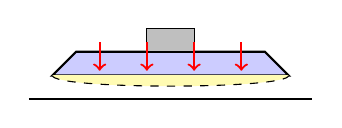
\begin{tikzpicture}[scale=0.6]
                % 船体
                \draw[fill=blue!20, thick] (-2,1) -- (2,1) -- (2.5,0.5) -- (-2.5,0.5) -- cycle;
                % 气垫
                \draw[fill=yellow!30, dashed] (-2.5,0.5) .. controls (-2.5,0.2) and (2.5,0.2) .. (2.5,0.5);
                % 地面
                \draw[thick] (-3,0) -- (3,0);
                % 风扇
                \draw[fill=gray!50] (-0.5,1) rectangle (0.5,1.5);
                % 气流箭头
                \foreach \x in {-1.5,-0.5,0.5,1.5}
                    \draw[->, thick, red] (\x,1.2) -- (\x,0.6);
            \end{tikzpicture}
            
            \small \textit{气垫悬浮原理}
        \end{center}
    \end{columns}
\end{frame}

% 第3页：系统架构
\begin{frame}{系统整体架构}
    \begin{center}
        
\includegraphics[width=0.55\textwidth]{mb.png}
        
        \vspace{0.3cm}
        \textit{主控制器硬件框图}
    \end{center}
    
    \vspace{-0.2cm}
    \begin{columns}
        \column{0.33\textwidth}
        \centering
        \textbf{感知层}
        \begin{itemize}
            \item MT9V034摄像头
            \item ICM-20602 IMU
            \item 电压监测
        \end{itemize}
        
        \column{0.33\textwidth}
        \centering
        \textbf{控制层}
        \begin{itemize}
            \item CH32V307主控
            \item FreeRTOS调度
            \item PID控制算法
        \end{itemize}
        
        \column{0.33\textwidth}
        \centering
        \textbf{执行层}
        \begin{itemize}
            \item 2×悬浮电机
            \item 4×推进电机
            \item CH32V203电调
        \end{itemize}
    \end{columns}
\end{frame}

% 第4页：核心硬件 - RISC-V芯片
\begin{frame}{核心硬件：RISC-V微控制器}
    \begin{columns}
        \column{0.5\textwidth}
        \textbf{主控芯片：CH32V307}
        \begin{itemize}
            \item \textcolor{blue}{RISC-V架构}，144MHz
            \item 256KB Flash，64KB SRAM
            \item 硬件浮点运算单元
            \item 丰富外设接口
        \end{itemize}
        
        \vspace{0.3cm}
        \begin{center}
            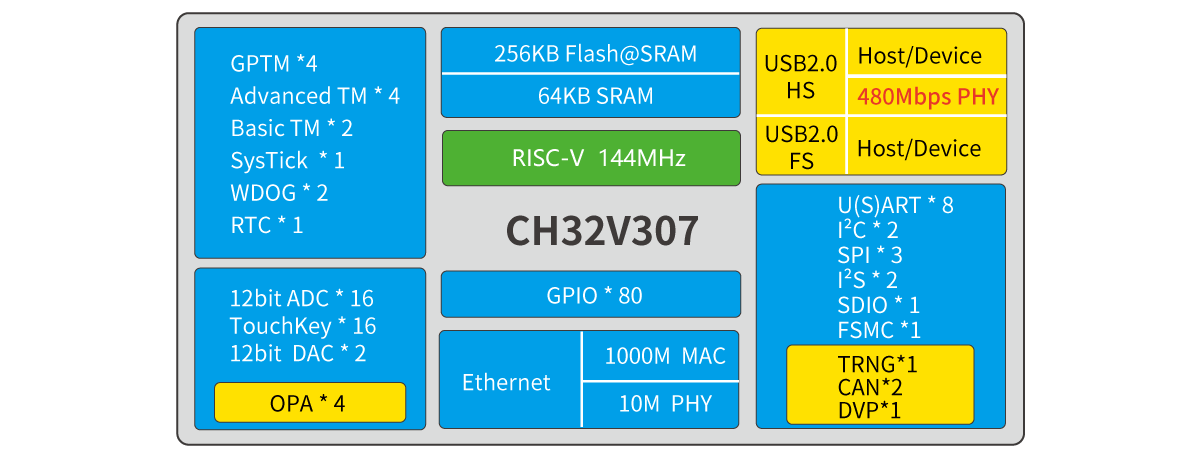
\includegraphics[width=0.7\textwidth]{ch32v307.png}
            
            \small \textit{CH32V307系统框图}
        \end{center}
        
        \column{0.5\textwidth}
        \textbf{电调芯片：CH32V203}
        \begin{itemize}
            \item RISC-V架构，144MHz
            \item 128KB Flash，64KB SRAM
            \item 高级定时器
            \item 互补PWM输出
        \end{itemize}
        
        \vspace{0.3cm}
        \begin{center}
            
\includegraphics[width=0.65\textwidth]{ch32.png}
            
            \small \textit{CH32V203系统框图}
        \end{center}
    \end{columns}
    
    \vspace{0.2cm}
    \begin{center}
        \textbf{优势：}开源指令集 + 自主可控 + 高性能实时响应
    \end{center}
\end{frame}

% 第5页：电机驱动系统
\begin{frame}{电机驱动系统}
    \begin{columns}
        \column{0.5\textwidth}
        \textbf{直流有刷驱动（H桥）：}
        \begin{itemize}
            \item AON7418功率MOSFET
            \item NCP81155栅极驱动
            \item 自举电路高侧驱动
            \item 硬件死区保护
        \end{itemize}
        
        \vspace{0.2cm}
        \begin{center}
            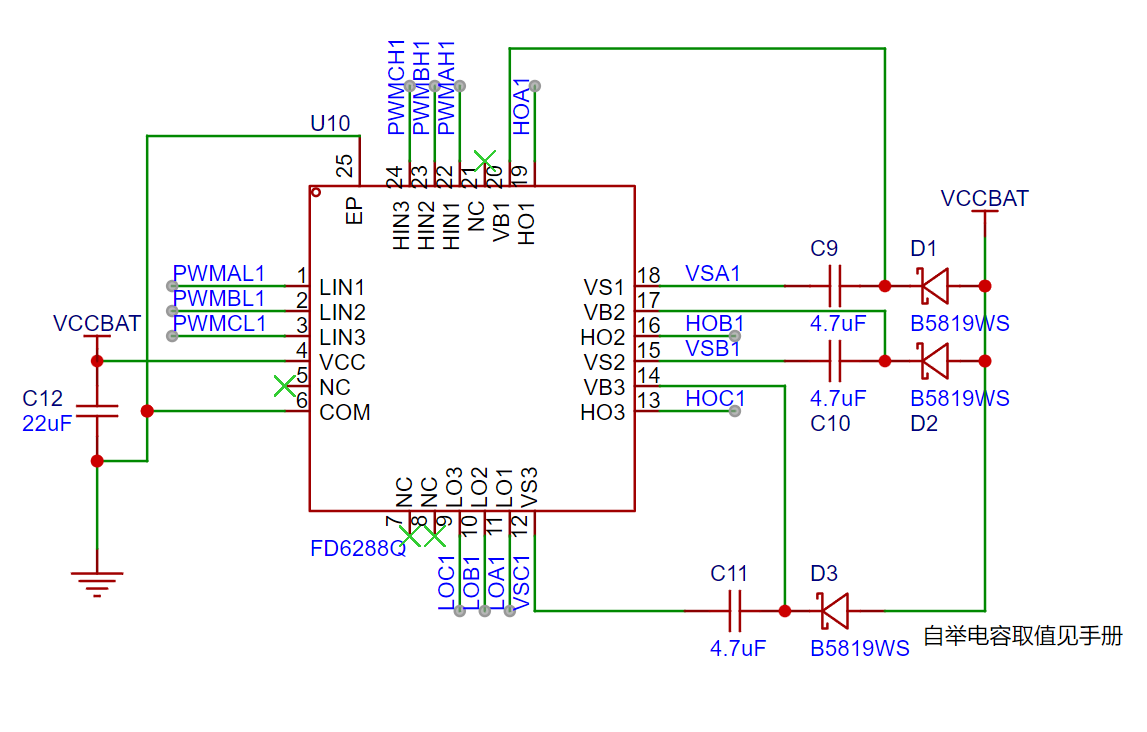
\includegraphics[width=0.9\textwidth]{fd6288q.png}
            
            \small \textit{栅极驱动电路}
        \end{center}
        
        \column{0.5\textwidth}
        \textbf{无刷电机驱动：}
        \begin{itemize}
            \item FD6288Q三相半桥驱动
            \item 反电势过零检测
            \item 六步换相控制
            \item 无需霍尔传感器
        \end{itemize}
        
        \vspace{0.2cm}
        \begin{center}
            
\includegraphics[width=0.8\textwidth]{dt.png}
            
            \small \textit{电调硬件框图}
        \end{center}
    \end{columns}
\end{frame}

% 第6页：无刷电机控制原理
\begin{frame}{无刷电机控制：六步换相法}
    \begin{columns}
        \column{0.45\textwidth}
        \textbf{工作原理：}
        \begin{itemize}
            \item 每步激活两个绕组
            \item 顺序产生旋转磁场
            \item 转一圈换相6次
        \end{itemize}
        
        \vspace{0.2cm}
        \textbf{过零检测：}
        \begin{center}
            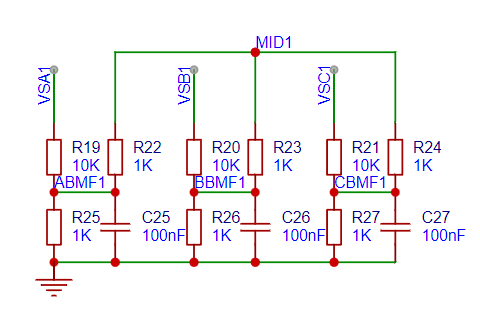
\includegraphics[width=0.95\textwidth]{vvv.png}
            
            \small \textit{反电势过零检测电路}
        \end{center}
        
        \column{0.55\textwidth}
        \textbf{六步换相时序：}
        \begin{center}
            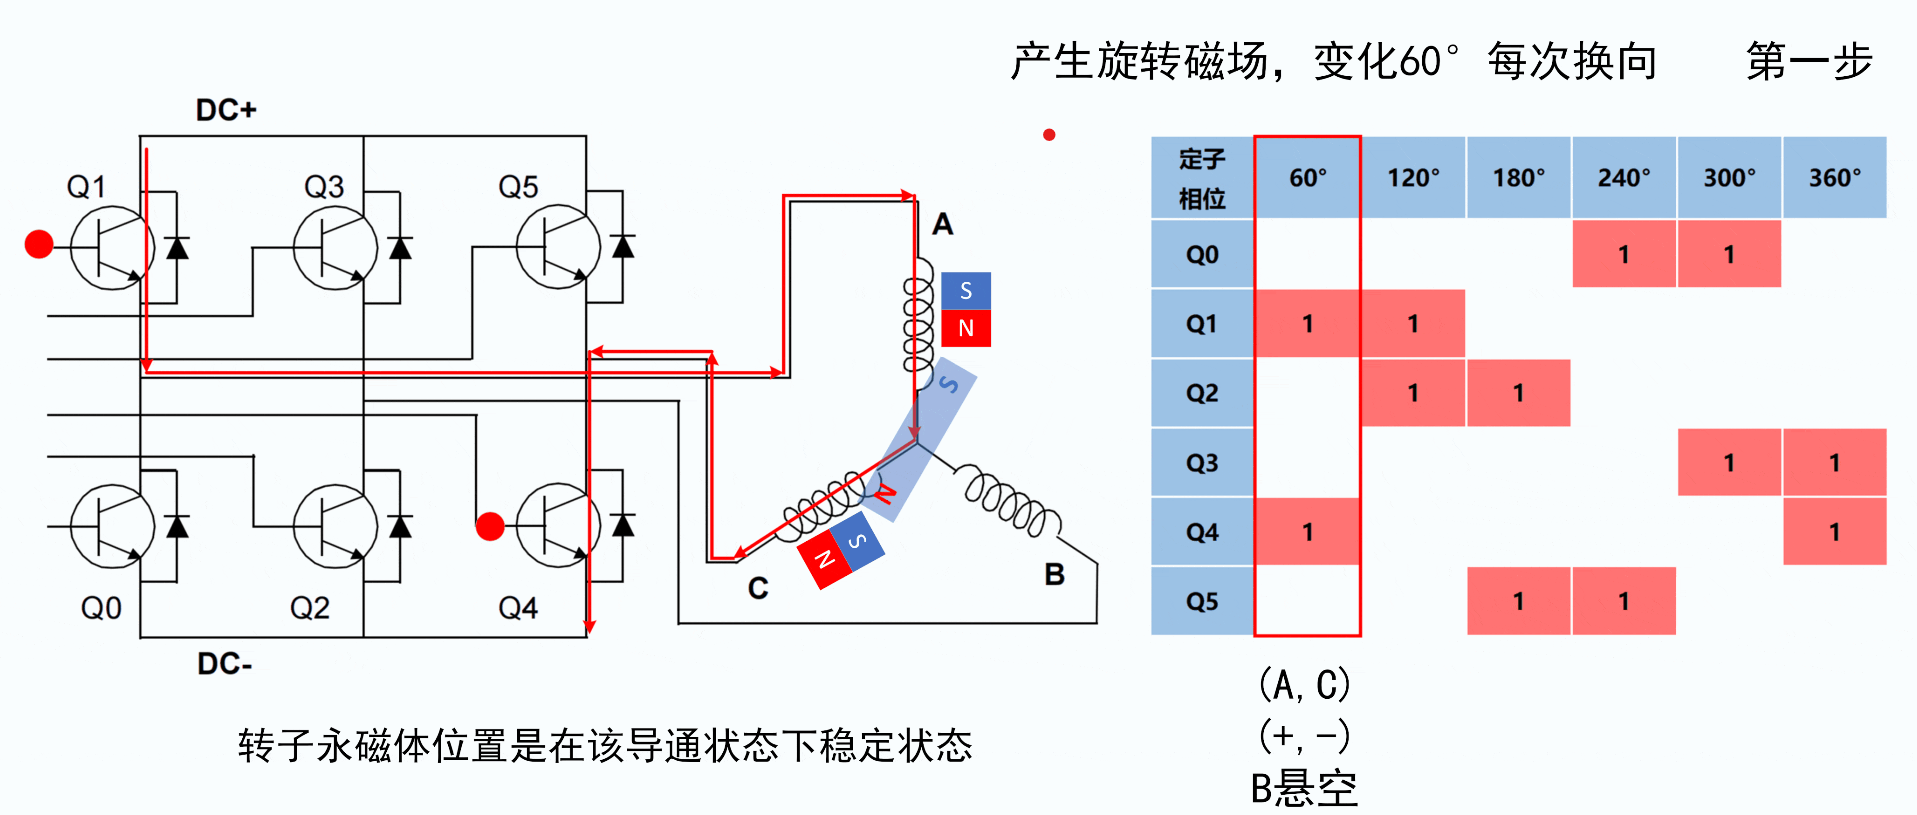
\includegraphics[width=0.28\textwidth]{liubu1.png}
            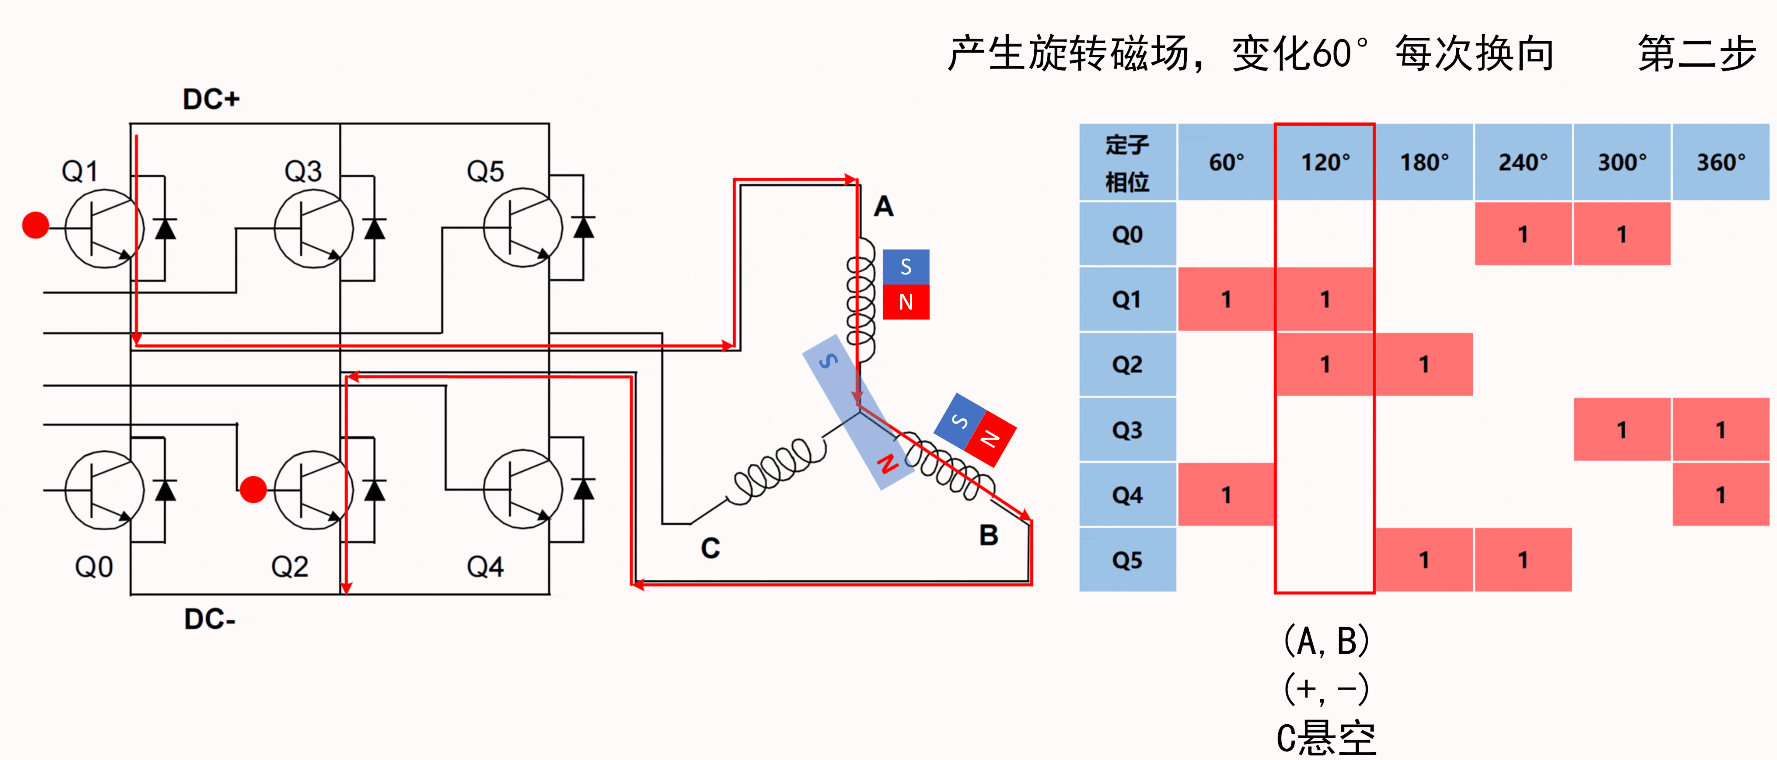
\includegraphics[width=0.28\textwidth]{liubu2.png}
            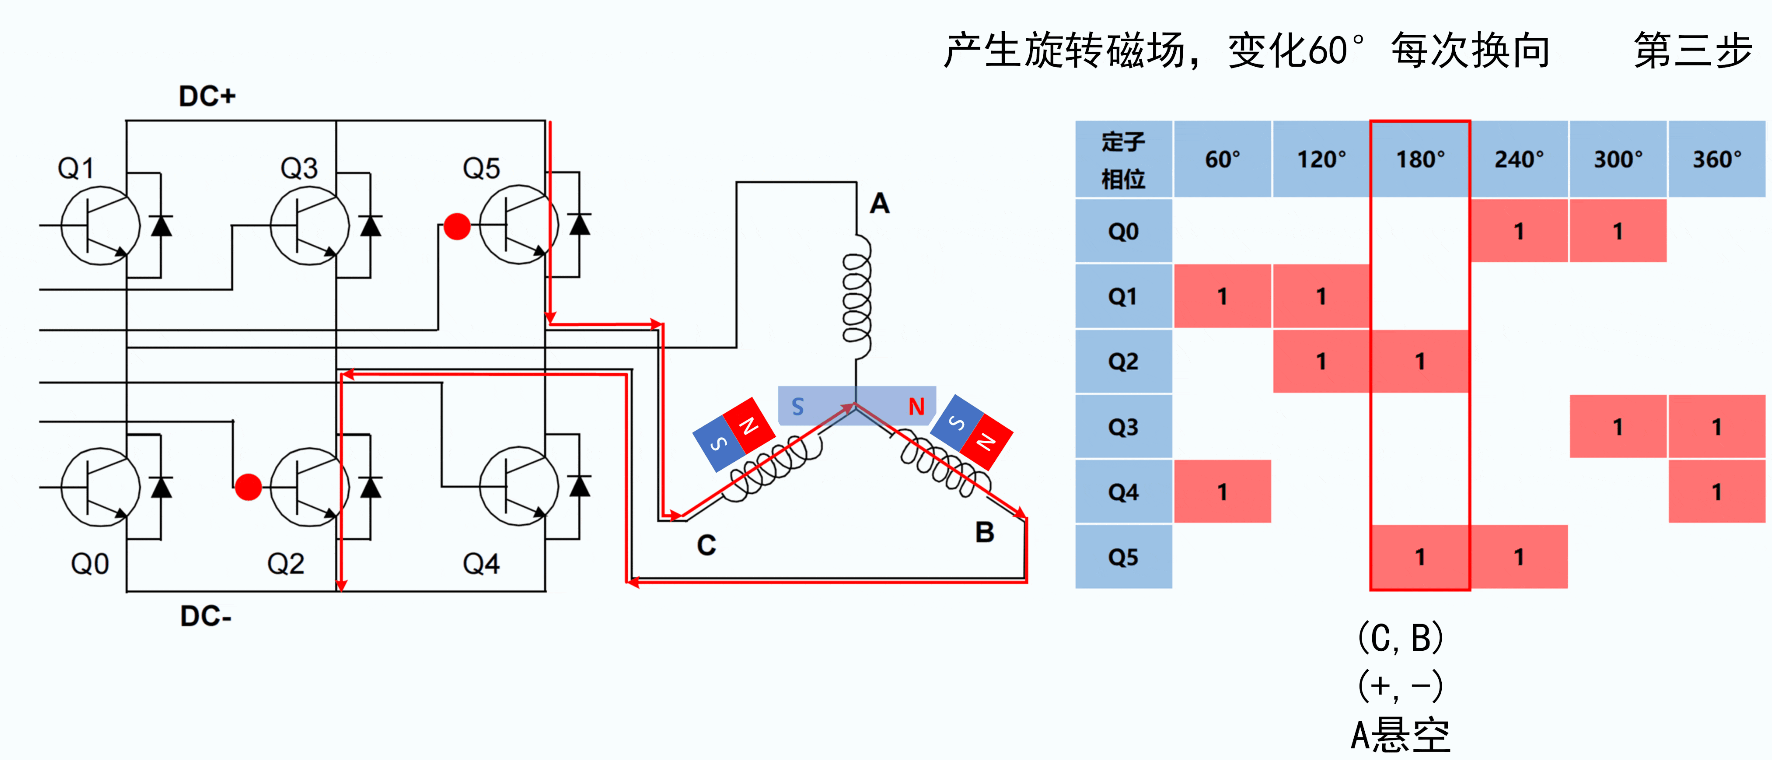
\includegraphics[width=0.28\textwidth]{liubu3.png}
            
            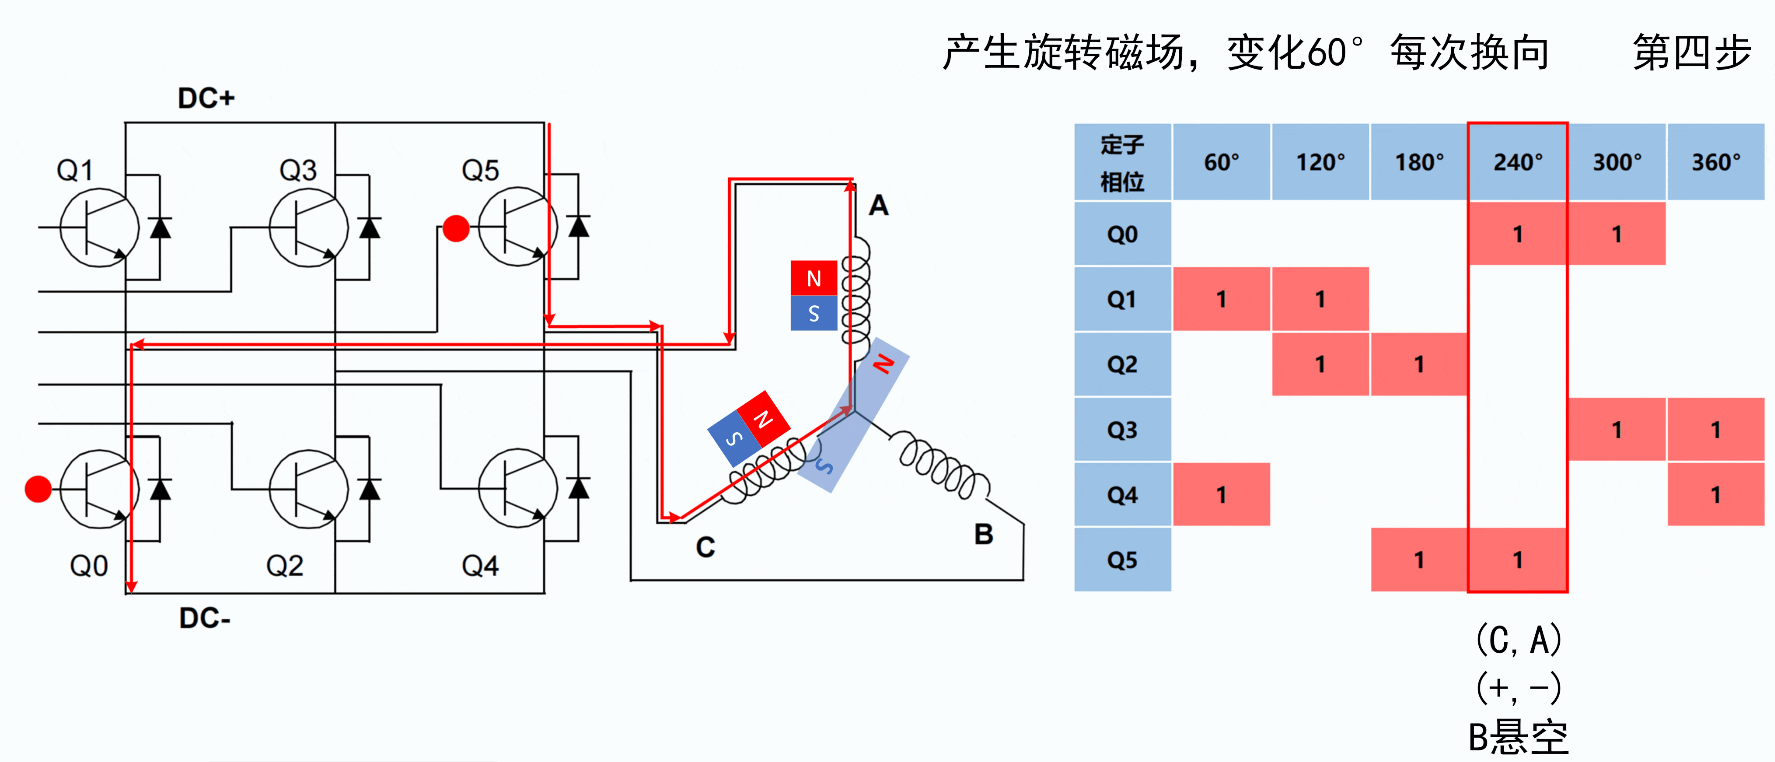
\includegraphics[width=0.28\textwidth]{liubu4.png}
            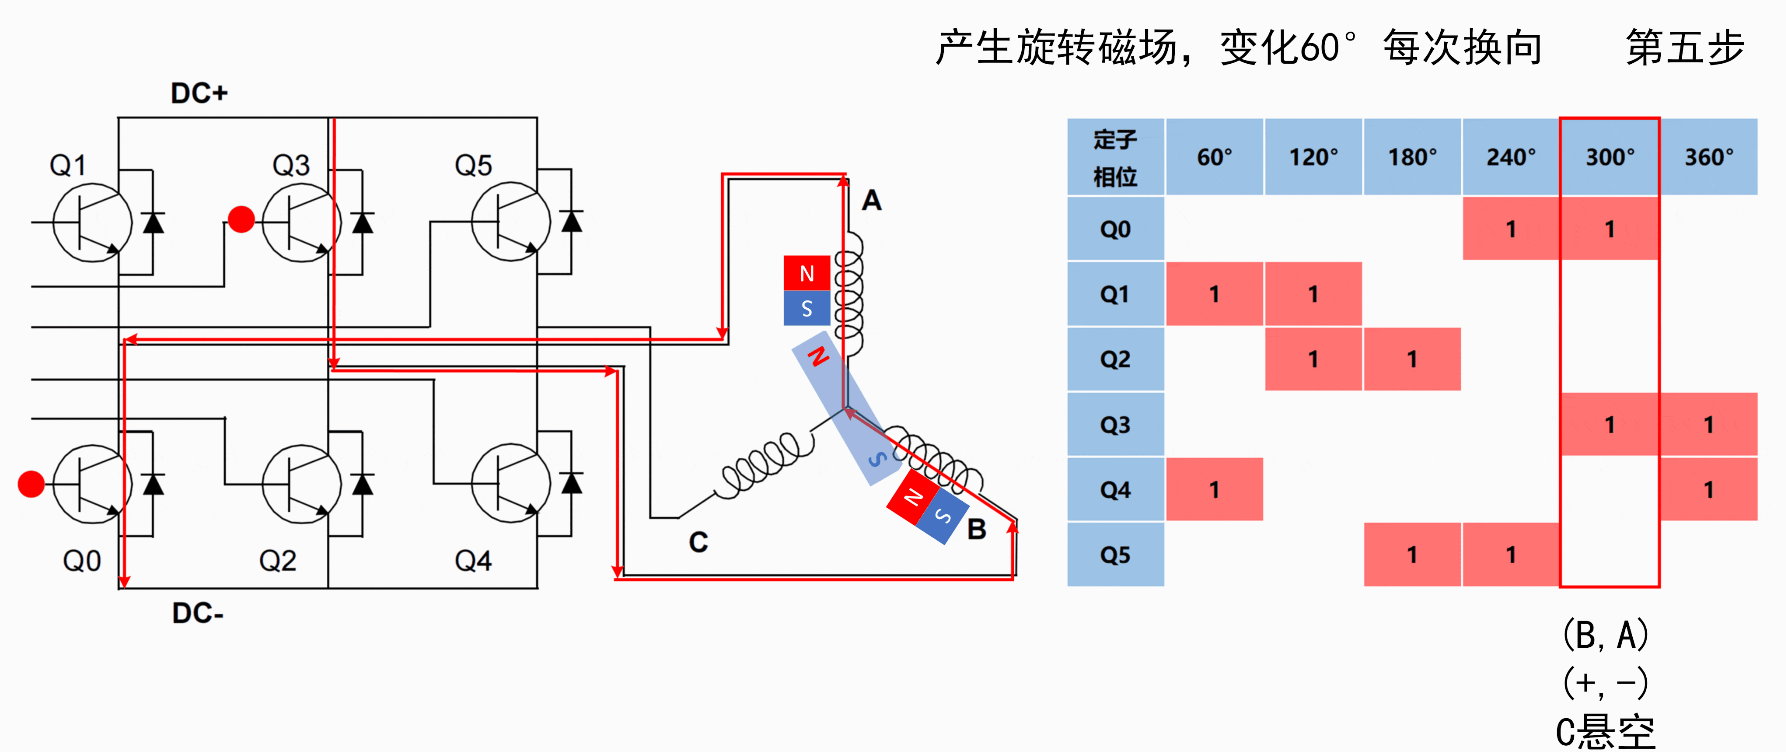
\includegraphics[width=0.28\textwidth]{liubu5.png}
            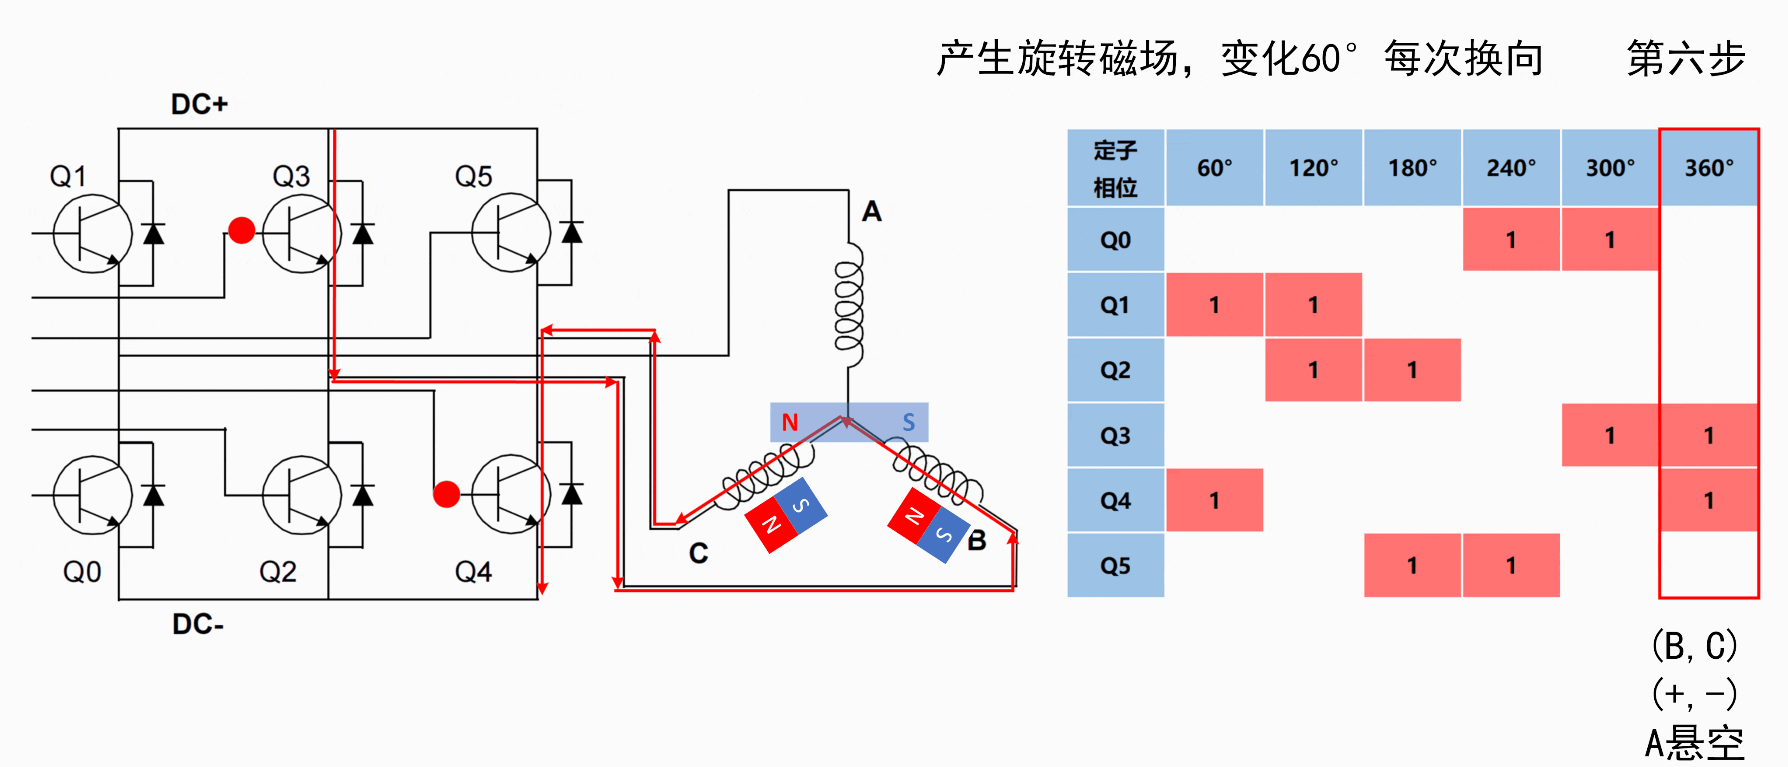
\includegraphics[width=0.28\textwidth]{liubu6.png}
            
            \small \textit{A-C → A-B → C-B → C-A → B-A → B-C}
        \end{center}
        
        \vspace{0.2cm}
        \small 虚拟中性点电压：$U_N' = \frac{U_A + U_B + U_C}{3}$
        
        \small 过零条件：$U_B = U_N' \Rightarrow E_B = 0$
    \end{columns}
\end{frame}

% 第7页：软件架构
\begin{frame}{软件系统架构}
    \begin{columns}
        \column{0.5\textwidth}
        \textbf{主控软件（FreeRTOS）：}
        \begin{center}
            
\includegraphics[width=0.5\textwidth]{c2.png}
        \end{center}
        
        \begin{itemize}
            \item 业务逻辑层
            \item 功能中间件层
            \item 硬件驱动层
        \end{itemize}
        
        \column{0.5\textwidth}
        \textbf{电调软件（裸机）：}
        \begin{center}
            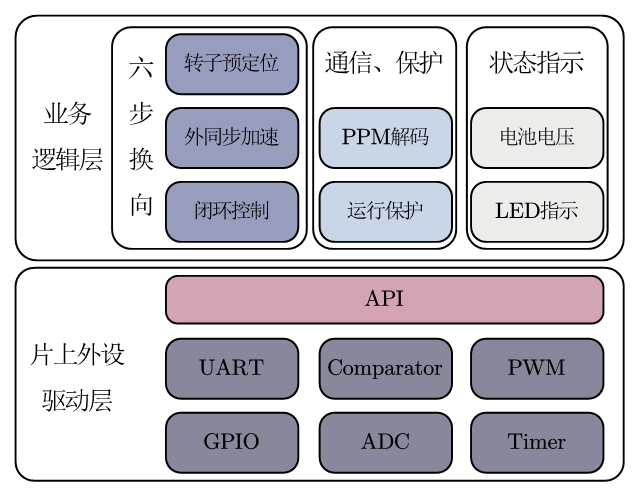
\includegraphics[width=0.5\textwidth]{c1.png}
        \end{center}
        
        \begin{itemize}
            \item 系统初始化
            \item PPM信号解码
            \item 六步换相控制
            \item 故障保护
        \end{itemize}
    \end{columns}
    
    \vspace{0.2cm}
    \begin{center}
        \textbf{核心算法：}PID控制 + 卡尔曼滤波 + 图像处理
    \end{center}
\end{frame}

% 第8页：控制算法
\begin{frame}{控制算法：混合PID策略}
    \begin{columns}
        \column{0.5\textwidth}
        \textbf{行进电机（串级PID）：}
        \begin{center}
            
\includegraphics[width=0.95\textwidth]{motor.png}
        \end{center}
        
        \begin{itemize}
            \item 外环：角度环
            \item 内环：角速度环
            \item 并级：速度环
        \end{itemize}
        
        \column{0.5\textwidth}
        \textbf{横向电机（位置式PID）：}
        \begin{center}
            
\includegraphics[width=0.95\textwidth]{motorside.png}
        \end{center}
        
        \begin{itemize}
            \item 基于图像偏差
            \item 提供向心力
            \item 快速转向
        \end{itemize}
    \end{columns}
    
    \vspace{0.2cm}
    \small \centering PID控制律：$u(t) = K_p e(t) + K_i \int_0^t e(\tau) d\tau + K_d \frac{de(t)}{dt}$
\end{frame}

% 第9页：姿态解算
\begin{frame}{姿态解算：卡尔曼滤波}
    \begin{columns}
        \column{0.6\textwidth}
        \textbf{算法流程：}
        
        \small
        \textbf{1. 预测步骤：}
        \begin{align*}
        \hat{x}_{k}^{-} &= A\hat{x}_{k-1} + Bu_{k-1} \\
        P_{k}^{-} &= AP_{k-1}A^T + Q
        \end{align*}
        
        \textbf{2. 更新步骤：}
        \begin{align*}
        K_k &= P_{k}^{-}H^T(HP_{k}^{-}H^T + R)^{-1} \\
        \hat{x}_k &= \hat{x}_{k}^{-} + K_k(z_k - H\hat{x}_{k}^{-}) \\
        P_k &= (I - K_kH)P_{k}^{-}
        \end{align*}
        
        \column{0.4\textwidth}
        \textbf{状态空间：}
        $X = \begin{bmatrix} \theta \\ \omega_b \end{bmatrix}$
        \begin{itemize}
            \item $\theta$：横滚角
            \item $\omega_b$：陀螺仪漂移
        \end{itemize}
        
        \vspace{0.3cm}
        \textbf{优势：}
        \begin{itemize}
            \item 融合加速度计和陀螺仪
            \item 抑制传感器噪声
            \item 补偿漂移
            \item 实时高精度
        \end{itemize}
        
        \vspace{0.3cm}
        \small \textit{流程：}
        $\hat{X}_{k-1} \xrightarrow{预测} \hat{X}_{k}^{-} \xrightarrow{更新} \hat{X}_{k}$
    \end{columns}
\end{frame}

% 第10页：总结
\begin{frame}{技术栈总结}
    \begin{columns}
        \column{0.5\textwidth}
        \textbf{完整技术栈：}
        
        \begin{enumerate}
            \item \textbf{硬件层}
            \begin{itemize}
                \item RISC-V双核架构
                \item 多电机驱动系统
                \item 多传感器融合
            \end{itemize}
            
            \item \textbf{驱动层}
            \begin{itemize}
                \item 外设驱动（SPI、UART、PWM）
                \item 电机控制接口
                \item 传感器数据采集
            \end{itemize}
            
            \item \textbf{算法层}
            \begin{itemize}
                \item PID控制器
                \item 卡尔曼滤波
                \item 图像处理（OTSU）
            \end{itemize}
            
            \item \textbf{应用层}
            \begin{itemize}
                \item FreeRTOS任务调度
                \item 人机交互界面
                \item 故障诊断保护
            \end{itemize}
        \end{enumerate}
        
        \column{0.5\textwidth}
        \textbf{性能指标：}
        
        \begin{center}
        \small
        \begin{tabular}{|c|c|}
        \hline
        \textbf{指标} & \textbf{达到值} \\
        \hline
        控制周期 & 5ms \\
        \hline
        姿态精度 & ±1.5° \\
        \hline
        最大速度 & 2.3 m/s \\
        \hline
        续航时间 & 45 min \\
        \hline
        响应时间 & 150ms \\
        \hline
        \end{tabular}
        \end{center}
        
        \vspace{0.3cm}
        \textbf{核心特点：}
        \begin{itemize}
            \item ✓ 开源自主可控
            \item ✓ 高性能实时控制
            \item ✓ 模块化设计
            \item ✓ 成本可控
        \end{itemize}
        
        \vspace{0.3cm}
        \begin{center}
            \textbf{应用场景：}智能车竞赛、两栖机器人、\\特殊环境巡检、教学平台
        \end{center}
    \end{columns}
\end{frame}

\end{document}